\chapter{Implementation}\label{ch:implementation}
In practice to implement the models described above, I have used AnyLogic software.
Specifically in this chapter I will show the various flowcharts and the more specific transitions that require further study.
\section{Buyer agent implementation}
Let's start with the implementation of the Buyer.
\begin{figure}[hbtp]
\caption{Buyer statechart}
\centering
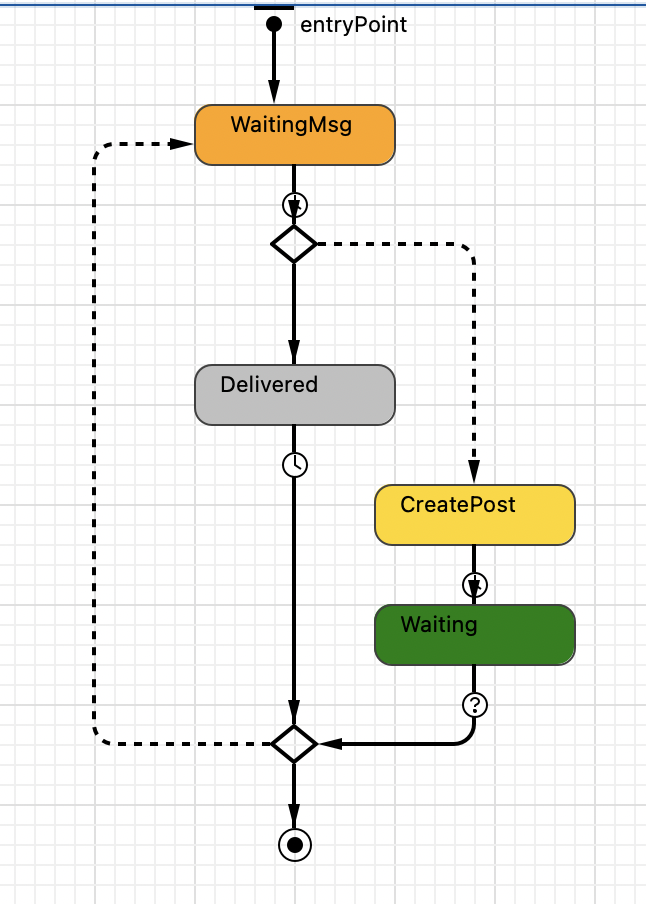
\includegraphics[scale=0.4]{../Images/buyerstatechart.png}
\end{figure}
The most important part to analyze is within the CreatePost state. In fact, there is some Java code here that is responsible for the operation of the orders.
\begin{lstlisting}[language=Java]
Post p = new Post();
p.buyer = this;
p.whoIs = 0;
p.numOfCloths = uniform_discr(1, 10);
p.postPrice = Math.round((uniform(0.5, 20) * p.numOfCloths) * 100.00) / 100.00;
post = p;
send(p, main.scheduler);
\end{lstlisting}
As you can see from the code I created a Post class where inside there are a number of attributes.
\begin{itemize}
\item \textbf{buyer}: who is the buyer and so in this case I pass him the \textbf{this} pointer, so himself being in the Buyer agent
\item \textbf{whoIs}: this is an integer attribute that allows me to figure out whether the order was placed by the Buyer (0) or the Worker (1)
\item \textbf{numOfCloths}: for the cloth numbers I relied on a Uniform Discrete random variable $\mathcal{U}$ of parameter $a = 1, b = 10$.
\item \textbf{postPrice}: same for post price by estimating on parameter b = 20
\item \textbf{status}: it's useful for understanding if the order is completed or is currently under working
\item \textbf{rider}: assign a rider for that specific post
\item \textbf{worker}: assign a worker for that specific post
\end{itemize}
This operation, on the other hand, must be commented out send(p, main.scheduler), since it is critical for handling the exchange of messages (and thus Posts).
Then the conditional transition are two: From the branch to delivered if the post (variable inside the Buyer agent) is not null and the status = 1.
\begin{lstlisting}
post != null && post.status ==  1
\end{lstlisting}
Same store from Waiting to the branch if status = 1.
\section{Scheduler agent implementation}
Another important agent is the Scheduler agent as we saw in the previous Chapter. However let's have a look inside the statechart.
\begin{figure}[hbtp]
\caption{Scheduler statechart}
\centering
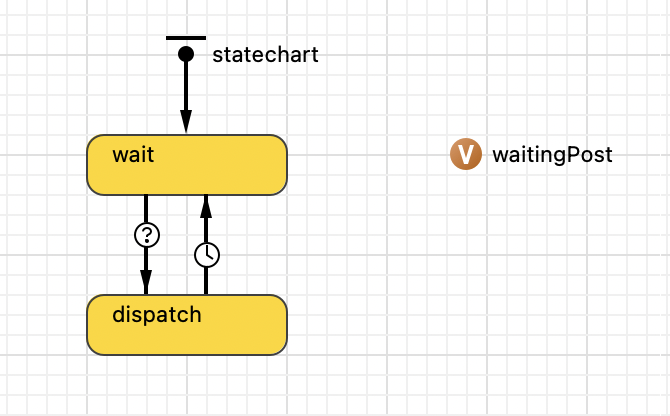
\includegraphics[scale=0.6]{../Images/schedulerstatechart.png}
\end{figure}
As you can see there are two transition in which one is conditional. Here the code for the trigger condition:
\begin{lstlisting}[language=Java]
waitingPost.size() > 0
\end{lstlisting}
so if the size of the queue isn't empty. Then if the condition is triggered there is this action to be executed:
\begin{lstlisting}[language=Java]
Post currPost = waitingPost.get(0);
waitingPost.remove(0);
if(currPost.whoIs == 0){
	Workers_iron w = main.workers_irons.findFirst(wi -> wi.inState(Workers_iron.Waiting));
	currPost.worker = w;
	Rider r = main.riders.findFirst(ri -> ri.inState(Rider.Waiting));
	if(r != null){
		currPost.rider = r;
		send(currPost,r);
	}
	
}else{
	Rider r = main.riders.findFirst(ri -> ri.inState(Rider.Waiting));
	if(r != null){
		currPost.rider = r;
		send(currPost,r);
	}
	
}
\end{lstlisting}
So I'll extract from the queue the first order and I remove it. Then I check if the order is from the Buyer, so it means that we need to search and find the first worker that is in the Waiting state, assign it to the Post attribute worker and the find the first rider that is in a Waiting state. If so, we assign the rider to the currentPost and then send currentPost to the rider. Instead, if the order is produced by the Worker, we just find a free rider that can take the processed order and send back to the Buyer. 
\section{Rider agent implementation}
In order to make the simulation work I need this agent. Here the statechart:
\begin{figure}[hbtp]
\caption{Rider statechart}
\centering
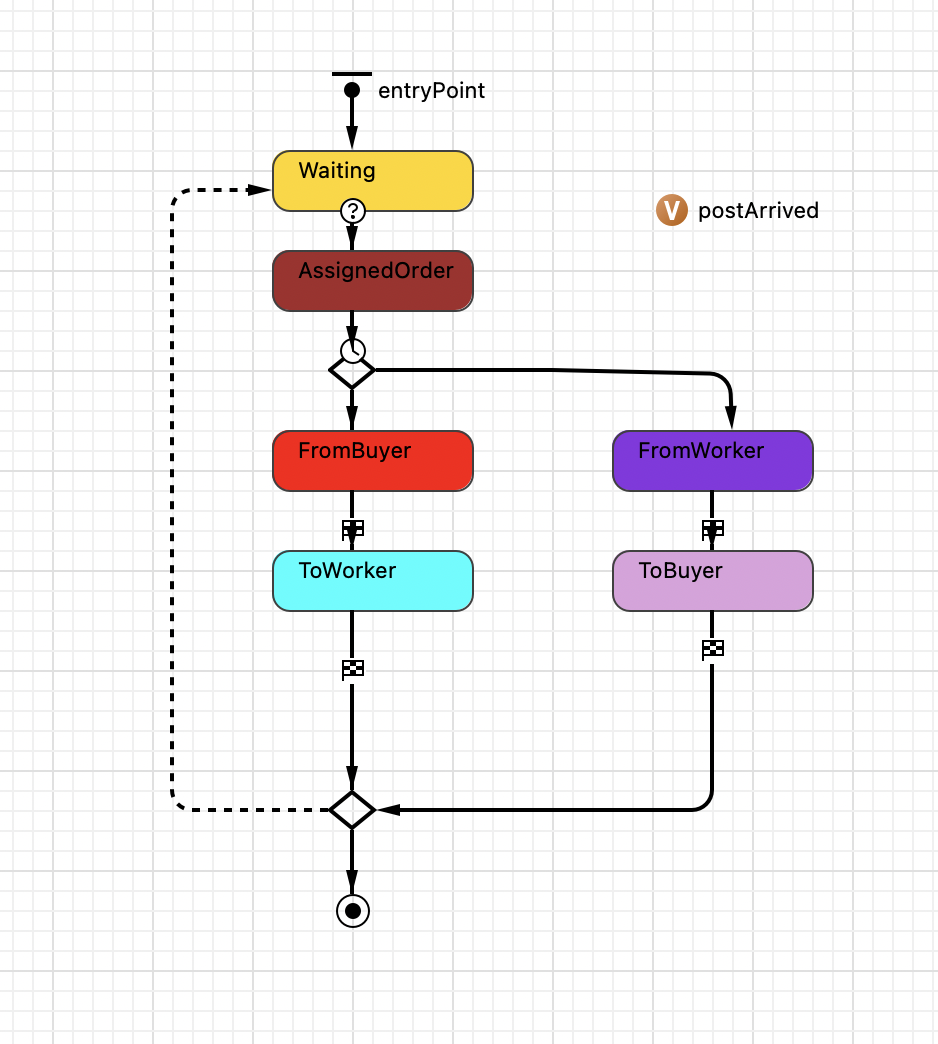
\includegraphics[scale=0.6]{../Images/riderstatechart.png}
\end{figure}
As we discussed previously the important thing here is to understand how the rider will move and how to trigger the conditions. Indeed we have two different flow: one is from \textbf{FromBuyer state} to \textbf{ToWorker state} state and here the rider will deliver the laundry from the Buyer to the Worker that need now to iron/wash his cloths. On the other hand we have the flow from \textbf{FromWorker state} to \textbf{ToBuyer state} that means that the Worker has finished his job and now the rider can catch the laundry and deliver to the owner (Buyer).
When the rider is the \textbf{AssignedOrder state} through the condition
\begin{lstlisting}[language=Java]
postArrived.whoIs == 0
\end{lstlisting} 
we execute this action 
\begin{lstlisting}[language=Java]
moveTo(postArrived.buyer);
\end{lstlisting} 
Note that each state block has his own color. That's useful to recognize in which state the rider enter during the simulation by change the shapeColor using this code:
\begin{lstlisting}[language=Java]
shapeBody.setFillColor(red);
\end{lstlisting} 
When the rider is arrived for example to the Buyer , he will pass in the other state like ToWorker state only by the transition that is trigger by agentArrival. (It is represented as a checkered flag). When this is true the action is the follow:
\begin{lstlisting}[language=Java]
moveTo(postArrived.worker); 
\end{lstlisting} 
Same story but in the opposite way for the other branch. After the deliver the rider will set the postArrived to null and with the Bernoulli random variable as discussed in the Model Chapter we can continue the flow.
\section{Worker agent implementation}
Then to complete the flow, we need the Worker agent that has the duty of complete the service that the Buyer asked. Here the statechart:
\begin{figure}[hbtp]
\caption{Worker\_iron statechart}
\centering
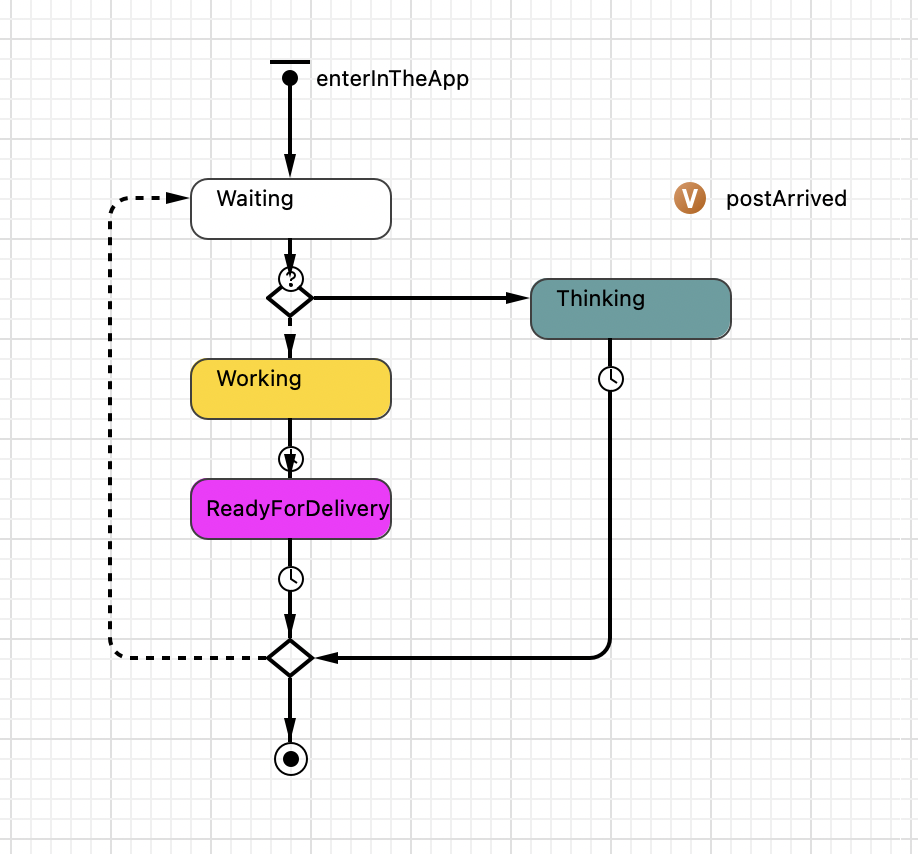
\includegraphics[scale=0.6]{../Images/workerstatechart.png}
\end{figure}
The only thing to discuss here is the conditional transition that allow us to enter inside the branch. Indeed:
\begin{lstlisting}[language=Java]
postArrived != null
\end{lstlisting} 
then the Worker can enter in the Working states otherwise he will enter in the Thinking state.
\section{Main agent implementation}
Finally let's talk about the special agent of the simulation that is called \textbf{Main agent}. It represents the "dashboard" of the simulation. 
\begin{figure}[hbtp]
\caption{Main agent }
\centering
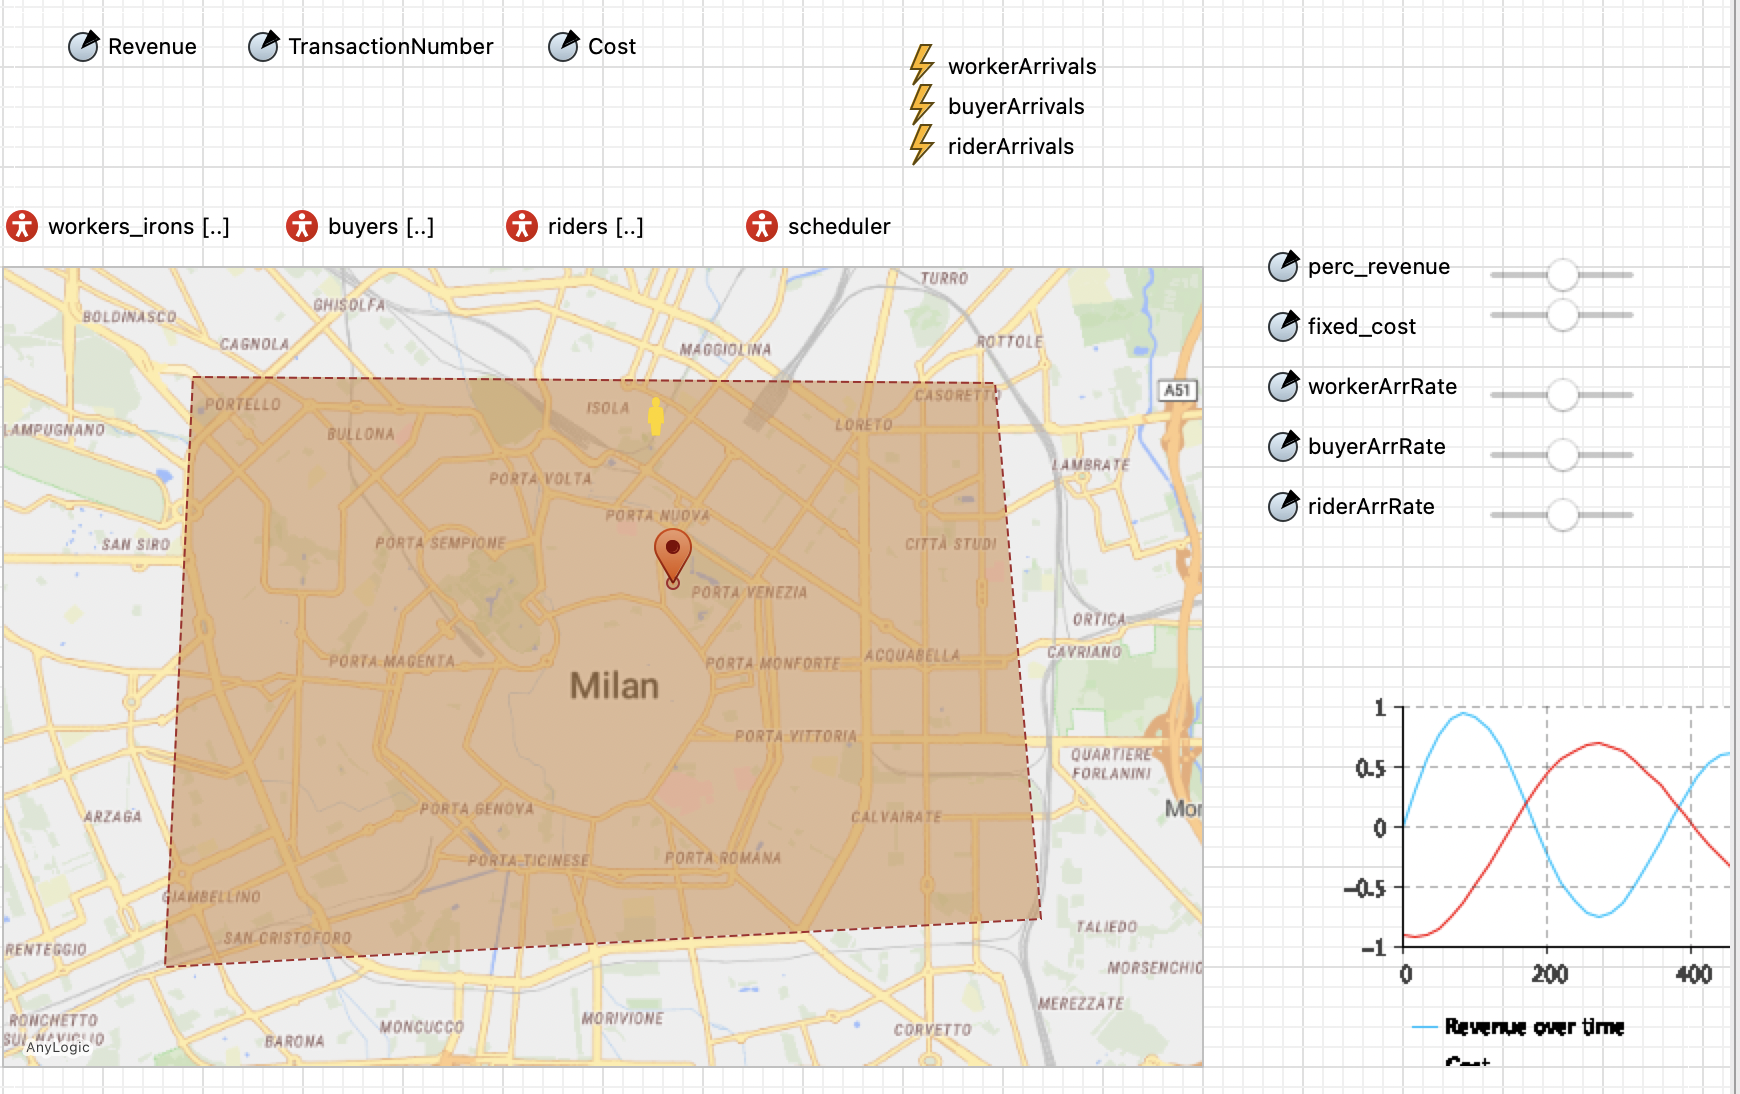
\includegraphics[scale=0.5]{../Images/main.png}
\end{figure}
As you can see the first thing that appear is the GIS map. It is centered in Milan, in which the simulation will run. With the help of the gis region I established a wide area within worker,buyer,rider can spawn. In the top-right corner there are 3 different arrivals, one for each agent, excluding the Scheduler.
With this code they can spawn in the GIS Region, just change the agent that we want to spawn:
\begin{lstlisting}[language=Java]
Rider r = add_riders();
Point p = gisRegion.randomPointInside();
Position q = new Position();
q.setLocation(p);
r.setPosition(q);
\end{lstlisting} 
Then let's consider the trigger type. They are all Rate and the amount is customizable with the sliders on the right side. Jusr riders are Rate/per day instead the other are Rate/per hours.
To conclude all are population of agents and just the scheduler is a single agent.
